\begin{exercise}
\begin{figure}[H]
\centering
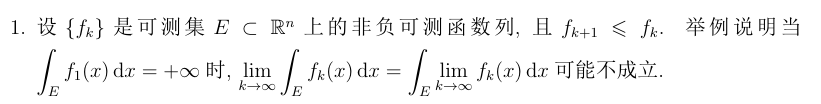
\includegraphics[width=\textwidth]{hw11-2025052017.png}
% \caption{}
\label{}
\end{figure}
\end{exercise}
\begin{proof}
When $E=\mathbb{R}$, $f_k\equiv\frac{1}{k}$,
\[
\lim_{ k \to \infty } \int_{E}^{} \underbrace{ f_k(x) }_{ =\frac{1}{k} } \, \mathrm{d}x =\lim_{ k \to \infty } \infty=\infty
\]
\[
\int_{E}^{} \lim_{ k \to \infty } \underbrace{ f_k(x) }_{ =\frac{1}{k} } \, \mathrm{d}x =\int_{E}^{} 0 \, \mathrm{d}x =0\neq \infty= \lim_{ k \to \infty } \int_{E}^{} f_k(x) \, \mathrm{d}x 
\]
\end{proof}

\begin{exercise}
\begin{figure}[H]
\centering
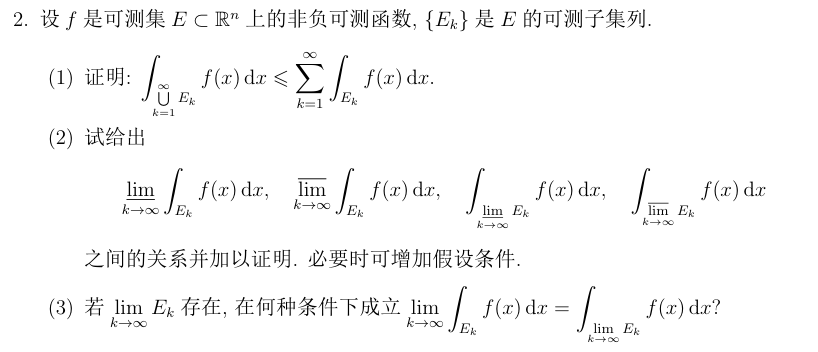
\includegraphics[width=\textwidth]{1-hw11-2025052017.png}
% \caption{}
\label{}
\end{figure}
\end{exercise}
\begin{proof}
(1)
\[
\begin{aligned}
\int_{\bigcup_{k=1}^{N} E_k}^{} f(x) \, \mathrm{d}x  & =\int_{E}^{} f(x)\cdot\chi_{\bigcup_{k=1}^{N} E_k}(x) \, \mathrm{d}x  \\
 & \leq \int_{E}^{}f(x)\cdot \sum_{k=1}^{N} \chi_{E_k}(x)  \, \mathrm{d}x  \\
 & =\sum_{k=1}^{N} \int_{E}^{} \underbrace{ f(x) }_{ \geq 0 }\chi_{E_k}(x) \, \mathrm{d}x  \\
 & \leq \sum_{k=1}^{\infty} \int_{E}^{} f(x)\chi_{E_k}(x)  \, \mathrm{d}x  \\
 & =\sum_{k=1}^{\infty} \int_{E_k}^{} f(x) \, \mathrm{d}x 
\end{aligned}
\]
Let $N\to \infty$, then
\[
\int_{\bigcup_{k=1}^{\infty} E_k}^{} f(x) \, \mathrm{d}x \leq \sum_{k=1}^{\infty} \int_{E_k}^{} f(x) \, \mathrm{d}x
\]
(2)
Claim that
\[
\chi_{\varliminf_{ k \to \infty } E_k}=\varliminf_{ k \to \infty } \chi _{E_k}
\]
Case 1: $\chi_{\lim_{k\to\infty}E_k}(x)=1$

If $\chi_{\underline{\lim}_{k\to\infty}E_k}(x)=1$, then by the definition of the indicator function, $x\in\underline{\lim}_{k\to\infty}E_k$.

By the definition of the limit inferior of sets, this means there exists a natural number $N_0$ such that for all $k\geq N_0,x\in E_k.$

If $x\in E_k$ for all $k\geq N_0$, then $\chi_{E_k}(x)=1$ for all $k\geq N_0.$

Now consider $\underline{\lim}_{k\to\infty}\chi_{E_k}(x)$:
\[
\underline{\lim}_{k\to\infty}\chi_{E_k}(x)=\sup_{n\geq1}(\inf_{k\geq n}\chi_{E_k}(x))
\]
For $n=N_0$, we have $\inf_{k\geq N_0}\chi_{E_k}(x).$ Since $\chi_{E_k}(x)=1$ for all $k\geq N_0$, the infimum of these values is 1.

So, $\inf_{k\geq N_0}\chi_{E_k}(x)=1.$

Then, $\sup_{n\geq1}(\inf_{k\geq n}\chi_{E_k}(x))$ must be at least 1. Since $\chi_{E_k}(x)$ values are at most 1, their infima and suprema are also at most 1.

Therefore, $\sup_{n\geq1}(\inf_{k\geq n}\chi_{E_k}(x))=1.$

Thus, if $\chi_{\underline{\lim}_{k\to\infty}E_k}(x)=1$, then $\underline{\lim}_{k\to\infty}\chi_{E_k}(x)=1.$

Case 2: $\chi_{\underline{\lim}_{k\to\infty}E_k}(x)=0$

If $\chi_{\underline{\lim}_{k\to\infty}E_k}(x)=0$, then $x\notin\underline{\lim}_{k\to\infty}E_k.$

By the definition of the limit inferior of sets, this means that for every natural number $n$, there exists some $k\geq n$ such that $x\notin E_k$.(ie, $x$ is not in all $E_k$ from any index $n$ onwards; for any $n$ we can find a later $E_k$ that does not contain $x).$

If for any $n$, there exists a $k\geq n$ such that $x\notin E_k$, then for any $n$, there exists a $k\geq n$ such that $\chi_{E_k}(x)=0.$

This implies that for any $n,\inf_{k\geq n}\chi_{E_k}(x)=0.$ (Because if the infimum were 1, all $\chi_{E_k}(x)$ for $k\geq n$ would have to be 1, which contradicts that there's one equal to 0)

Now consider $\underline{\lim}_{k\to\infty}\chi_{E_k}(x):$
\[
\underline{\lim}_{k\to\infty}\chi_{E_k}(x)=\sup_{n\geq1}(\inf_{k\geq n}\chi_{E_k}(x))
\]
Since $\inf_{k\geq n}\chi_{E_k}(x)=0$ for all $n\geq1$, the supremum of a sequence of zeros is 0.

So, $\sup_{n\geq1}(0)=0.$

Thus, if $\chi_{\underline{\lim}_{k\to\infty}E_k}(x)=0$, then $\underline{\lim}_{k\to\infty}\chi_{E_k}(x)=0.$


By Fatou's lemma,
\[
\begin{aligned}
\int_{\varliminf_{ k \to \infty } E_k} f(x) \, \mathrm{d}x  & =\int_{E}^{} f(x)\cdot \chi_{\varliminf_{ k \to \infty } E_k}(x) \, \mathrm{d}x  \\
 & =\int_{E}^{} \varliminf_{ k \to \infty } f(x)\cdot \chi_{E_k}(x) \, \mathrm{d}x  \\
 & \leq \varliminf_{ k \to \infty } \int_{E}^{} f(x)\cdot \chi_{E_k}(x) \, \mathrm{d}x  \\
 & =\varliminf_{ k \to \infty } \int_{E_k}^{} f(x) \, \mathrm{d}x 
\end{aligned}
\]
Similarly,
\[
\varlimsup_{ k \to \infty } \int_{E_k}^{} f(x) \, \mathrm{d}x \leq  \int_{\varlimsup_{ k \to \infty } E_k}^{} f(x) \, \mathrm{d}x 
\]
Hence,
\begin{equation}
\int_{\varliminf_{ k \to \infty } E_k}^{} f(x) \, \mathrm{d}x \leq\varliminf_{ k \to \infty } \int_{E_k}^{} f(x) \, \mathrm{d}x \leq \varlimsup_{ k \to \infty } \int_{E_k}^{} f(x) \, \mathrm{d}x \leq  \int_{\varlimsup_{ k \to \infty } E_k}^{} f(x) \, \mathrm{d}x
\label{94ba73}
\end{equation}

(3)
As $\lim_{ k \to \infty }E_k$ exists, by \cref{94ba73},
\[
\lim_{ k \to \infty } \int_{E_k}^{} f(x) \, \mathrm{d}x =\int_{\lim_{ k \to \infty }E_k }^{} f(x) \, \mathrm{d}x
\]
\end{proof}

\begin{exercise}
\begin{figure}[H]
\centering
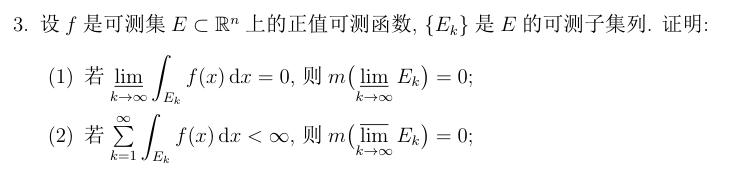
\includegraphics[width=\textwidth]{2-hw11-2025052017.png}
% \caption{}
\label{}
\end{figure}
\end{exercise}
\begin{proof}
(1)
By \cref{94ba73}, if $m(\varliminf_{ k \to \infty }E_k)>0$,
\[
\varliminf_{ k \to \infty } \int_{E_k}^{} f(x) \, \mathrm{d}x \geq \int_{\varliminf_{ k \to \infty } E_k}^{} f(x) \, \mathrm{d}x >0
\]
which is a contradiction.

(2)
If $m(\varlimsup_{ k \to \infty }E_k)>0$,
\[
 \int_{\bigcup_{k=N}^{\infty} E_k}^{}f(x)  \, \mathrm{d}x \leq \sum_{k=N}^{\infty}\int_{E_k}^{} f(x) \, \mathrm{d}x  
\]
Then
\[
0=\lim_{ N \to \infty } \sum_{k=N}^{\infty} \int_{E_k}^{} f(x) \, \mathrm{d}x \geq \lim_{ N \to \infty } \int_{\bigcup_{k=N}^{\infty} E_k}^{} f(x) \, \mathrm{d}x =\int_{\varlimsup_{ k \to \infty } E_k}^{} f(x) \, \mathrm{d}x>0
\]
which is a contradiction.

\begin{exercise}
\begin{figure}[H]
\centering
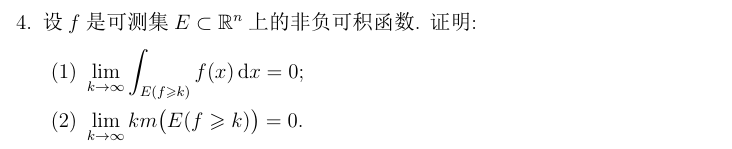
\includegraphics[width=\textwidth]{3-hw11-2025052017.png}
% \caption{}
\label{}
\end{figure}
\end{exercise}
(1)
\[
0\leq \varlimsup_{ k \to \infty } \int_{E(f\geq k)}^{} f(x) \, \mathrm{d}x \leq \int_{\varlimsup_{ k \to \infty } E(f\geq k)}^{} f(x) \, \mathrm{d}x =\int_{E(f=+\infty)}^{} f(x) \, \mathrm{d}x =0
\]
(2)
\[
km(E(f\geq k))\leq \int_{E(f\geq k)}^{} f(x) \, \mathrm{d}x
\]
Let $k\to \infty$, then
\[
0\leq \varlimsup_{ k \to \infty } km(E(f\geq k))\leq \varlimsup_{ k \to \infty } \int_{E(f\geq k)}^{} f(x) \, \mathrm{d}x =0
\]
Thus
\[
\lim_{ k \to \infty } km(E(f\geq k))=0
\]
\end{proof}

\begin{exercise}
\begin{figure}[H]
\centering
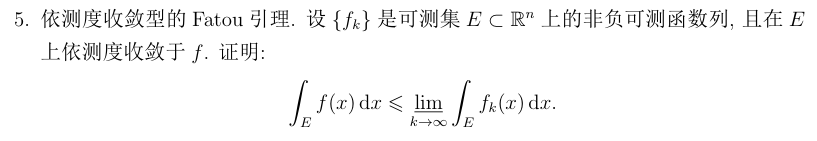
\includegraphics[width=\textwidth]{4-hw11-2025052017.png}
% \caption{}
\label{}
\end{figure}\label{5b171e}
\end{exercise}

\begin{proof}
By the definition of $\varliminf_{ k \to \infty }$, there exists $\{ k_{i} \}_{i\geq1}$ s.t.
\[
\lim_{ i \to \infty } \int_{E}^{} f_{k_i} (x)\, \mathrm{d}x=\varliminf_{ k \to \infty } \int_{E}^{} f_k (x)\, \mathrm{d}x  
\]
$f_k\overset{ m }{ \to }f$, then $f_{k_{i}}\overset{ m }{ \to }f$, thus there exists $\{ k_{i_{n}} \}_{n\geq1}$ s.t. $f_{k_{i_{n}}}\to f$ a.e. by Fatou's lemma,
\[
\int_{E}^{} f(x) \, \mathrm{d}x =\int_{E}^{} \varliminf_{ n \to \infty }  f_{k_{i_n}}(x) \, \mathrm{d}x \leq \varliminf_{ n \to \infty } \int_{E}^{} f_{k_{i_{n}}}(x) \, \mathrm{d}x =\lim_{ i \to \infty } \int_{E}^{} f_{k_i}(x) \, \mathrm{d}x =\varliminf_{ k \to \infty } \int_{E}^{} f_k(x) \, \mathrm{d}x
\]
\end{proof}

\begin{exercise}
\begin{figure}[H]
\centering
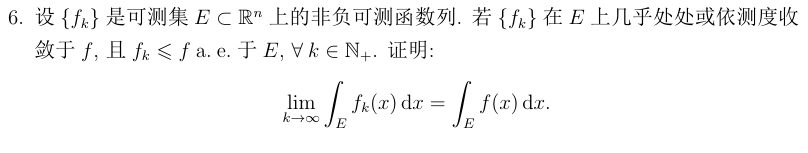
\includegraphics[width=\textwidth]{5-hw11-2025052017.png}
% \caption{}
\label{}
\end{figure}
\end{exercise}
\begin{proof}
By \cref{5b171e} ,
\[
\int_{E}^{} f(x) \, \mathrm{d}x \leq \varliminf_{ k \to \infty } \int_{E}^{} f_k(x) \, \mathrm{d}x
\]
As $f_k\leq f$ a.e. on $E$,
\[
\int_{E}^{} f(x) \, \mathrm{d}x \leq \varliminf_{ k \to \infty } \int_{E}^{} f_k(x) \, \mathrm{d}x \leq \int_{E}^{} f(x) \, \mathrm{d}x
\]
Then
\[
\int_{E}^{} f(x) \, \mathrm{d}x =\varliminf_{ k \to \infty } \int_{E}^{} f_k(x) \, \mathrm{d}x
\]
On the other hand, as $f_k\leq f$ a.e., we have
\[
\varlimsup_{ k \to \infty } \int_{E}^{} f_k(x) \, \mathrm{d}x \leq \varlimsup_{ k \to \infty } \int_{E}^{} f(x) \, \mathrm{d}x =\int_{E}^{} f(x) \, \mathrm{d}x \leq \varliminf_{ k \to \infty } \int_{E}^{} f_k(x) \, \mathrm{d}x
\]
Thus
\[
\lim_{ k \to \infty } \int_{E}^{} f_k(x) \, \mathrm{d}x
\]
exists.
\[
\lim_{ k \to \infty } \int_{E}^{} f_k(x) \, \mathrm{d}x =\int_{E}^{} f(x) \, \mathrm{d}x
\]
\end{proof}

\begin{exercise}
\begin{figure}[H]
\centering
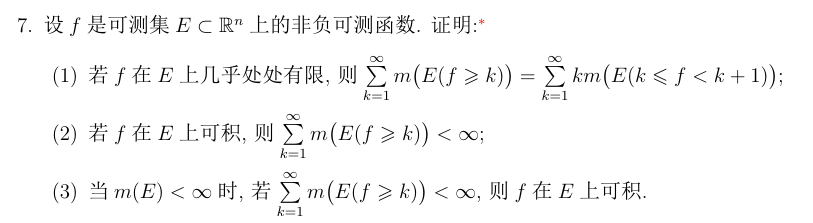
\includegraphics[width=\textwidth]{6-hw11-2025052017.png}
% \caption{}
\label{}
\end{figure}
\end{exercise}
\begin{proof}
(1)
\[
\begin{aligned}
\sum_{k=1}^{N} km(E(k\leq f<k+1)) & =\sum_{k=1}^{N} m(E(k\leq f<N+1))  \\
 & \leq \sum_{k=1}^{N} m(E(f\geq k)) 
\end{aligned}
\]
Let $N\to \infty$ then
\[
\sum_{k=1}^{\infty}km(E(k\leq f<k+1))\leq \sum_{k=1}^{\infty} m(E(f\geq k))
\]
On the other hand, since $m(E(f=\infty))=0$,
\[
\begin{aligned}
\sum_{k=1}^{N} m(E(f\geq k)) & =\sum_{k=1}^{N} \sum_{m=0}^{\infty} \underbrace{ m(E(k+m\leq f<k+m+1)) }_{ \geq 0 } \\
 & \overset{ \text{Tonelli} }{ = }\sum_{m=0}^{\infty} \sum_{k=1}^{N} m(E(k+m\leq f<k+m+1)) \\
 & =\sum_{i=1}^{\infty} \underbrace{ \#\{ (m,k):m+k=i,m\in \{ 0,\dots,\infty \},k\in \{ 1,\dots,N \} \} }_{ =\begin{cases}
i  & \text{when }i\leq N\\
N &  \text{when }i\geq N+1
\end{cases} }\cdot m(E(i\leq f<i+1)) \\
 & \leq \sum_{i=1}^{\infty} i\cdot m(E(i\leq f<i+1)) 
\end{aligned}
\]
Let $N\to \infty$, then
\[
\sum_{k=1}^{\infty} m(E(f\geq k))\leq \sum_{k=1}^{\infty} k\cdot m(E(k\leq f<k+1))
\]
Hence,
\[
\sum_{k=1}^{\infty} m(E(f\geq k))= \sum_{k=1}^{\infty} k\cdot m(E(k\leq f<k+1))
\]
(2)
\[
\int_{E}^{} f(x) \, \mathrm{d}x <\infty
\]
As $f$ is integrable, $f$ is finite a.e.
\[
\begin{aligned}
\int_{E}^{} f(x) \, \mathrm{d}x  & =\int_{E}^{} f(x)\cdot \chi_{\bigsqcup _{k=1}^{\infty} E(k\leq f<k+1)}(x) \, \mathrm{d}x  \\
 & =\int_{E}^{} \sum_{k=1}^{\infty} f(x)\cdot \chi_{E(k\leq f<k+1)}(x) \, \mathrm{d}x  \\
 & \overset{ \text{LDT} }{ = }\sum_{k=1}^{\infty } \int_{E(k\leq f<k+1)}^{} f(x) \, \mathrm{d}x  \\
 & \geq \sum_{k=1}^{\infty} \int_{E(k\leq f<k+1)}^{} k \, \mathrm{d}x  \\
 & =\sum_{k=1}^{\infty} k\cdot m(E(k\leq f<k+1))  \\
 & =\sum_{k=1}^{\infty} m(E(f\geq k))
\end{aligned}
\]
Therefore
\[
\sum_{k=1}^{\infty} m(E(f\geq k))<\infty
\]
(3)
\[
\int_{E}^{} f(x) \, \mathrm{d}x \leq \sum_{k=1}^{\infty} (k+1)\cdot m(E(k\leq f<k+1))=\sum_{k=1}^{\infty} m(E(f\geq k))+m(E)<\infty
\]
\end{proof}

\begin{exercise}
\begin{figure}[H]
\centering
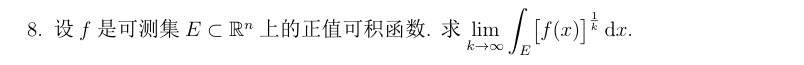
\includegraphics[width=\textwidth]{7-hw11-2025052017.png}
% \caption{}
\label{}
\end{figure}
\end{exercise}
\begin{proof}
For $x\in E$, we have $f(x)>0$, thus $\lim_{ k \to \infty }[f(x)]^{1/k}=1$. We need to show that
\[
\lim_{ k \to \infty } \int_{E}^{} [f(x)]^{1/k } \, \mathrm{d}x =m(E)
\]
By Levi's theorem,
\[
\lim_{ k \to \infty } \int_{E(f\leq 1)}^{} [f(x)]^{\frac{1}{k}} \, \mathrm{d}x =\int_{E(f\leq 1)}^{} \lim_{ k \to \infty } [f(x)]^{\frac{1}{k}} \, \mathrm{d}x=m(E(f\leq 1))
\]
If $m(E)=\infty$, then $m(E(f\leq1))=\infty$ or $m(E(f>1))=\infty$. If $m(E(f\leq1))=\infty$, then
\[
\lim_{ k \to \infty } \int_{E}^{} [f(x)]^{\frac{1}{k}} \, \mathrm{d}x \geq \lim_{ k \to \infty } \int_{E(f\leq 1)}^{} [f(x)]^{\frac{1}{k}} \, \mathrm{d}x =\infty
\]
Thus
\[
m(E)=\infty=\lim_{ k \to \infty } \int_{E}^{} [f(x)]^{\frac{1}{k}} \, \mathrm{d}x
\]
If $m(E(f>1))=\infty$, then
\[
\lim_{ k \to \infty } \int_{E}^{} [f(x)]^{\frac{1}{k}} \, \mathrm{d}x \geq \lim_{ k \to \infty } \int_{E(f>1)}^{} [f(x)]^{\frac{1}{k}} \, \mathrm{d}x \geq \int_{E(f>1)}^{} 1 \, \mathrm{d}x =m(E(f>1))=\infty
\]
Thus
\[
m(E)=\infty=\lim_{ k \to \infty } \int_{E}^{} [f(x)]^{\frac{1}{k}} \, \mathrm{d}x
\]
If $m(E)<\infty$, then for $k>1$, $[f(x)]^{\frac{1}{k}}\leq f(x)$ for any $x\in E(f>1)$, $[f(x)]^{\frac{1}{k}}$ is integrable on $E(f>1)$. By Lebesgue dominant theorem,
\[
\lim_{ k \to \infty } \int_{E(f>1)}^{} [f(x)]^{\frac{1}{k}} \, \mathrm{d}x =\int_{E(f>1)}^{} \lim_{ k \to \infty } [f(x)]^{\frac{1}{k}} \, \mathrm{d}x =\int_{E(f>1)}^{} 1 \, \mathrm{d}x =m(E(f>1))
\]
Then
\[
\begin{aligned}
\lim_{ k \to \infty } \int_{E}^{} [f(x)]^{\frac{1}{k}} \, \mathrm{d}x  & =\lim_{ k \to \infty } \int_{E(f\leq 1)}^{} [f(x)]^{\frac{1}{k}} \, \mathrm{d}x +\lim_{ k \to \infty } \int_{E(f>1)}^{} [f(x)]^{\frac{1}{k}} \, \mathrm{d}x  \\
 & =m(E(f\leq 1))+m(E(f>1)) \\
 & =m(E)
\end{aligned}
\]
\end{proof}

\begin{exercise}
\begin{figure}[H]
\centering
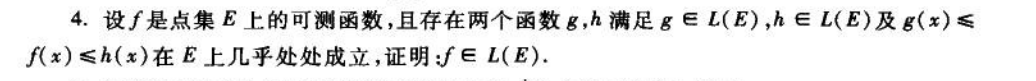
\includegraphics[width=\textwidth]{8-hw11-2025052017.png}
% \caption{}
\label{}
\end{figure}
\end{exercise}
\begin{proof}
\[
-\infty<\int_{E}^{} g(x) \, \mathrm{d}x \leq \int_{E}^{} f(x) \, \mathrm{d}x \leq \int_{E}^{} h(x) \, \mathrm{d}x <+\infty
\]
Hence $f\in L(E)$.
\end{proof}

\begin{exercise}
\begin{figure}[H]
\centering
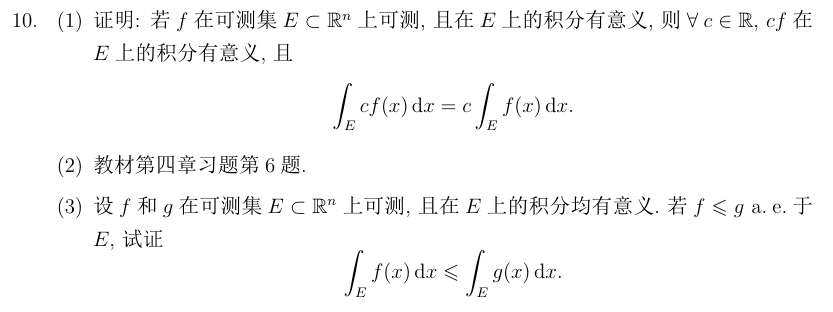
\includegraphics[width=\textwidth]{9-hw11-2025052017.png}
% \caption{}
\label{}
\end{figure}
\begin{figure}[H]
\centering
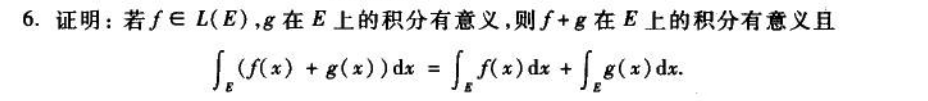
\includegraphics[width=\textwidth]{hw11-2025052023.png}
% \caption{}
\label{}
\end{figure}
\end{exercise}
\begin{proof}
(1)
The integration of $f$ is defined as
\[
\int_{E}^{} f  =\int_{E}^{} f^{+}  -\int_{E}^{} f^{-} 
\]
It makes sense iff the integration of $f^{+}$ and $f^{-}$ make sense. WLOG, we suppose that $f$ is nonnegative. For $c>0$, $0\leq h\leq f$ on $E$ iff $0\leq ch\leq cf$ on $E$. Therefore, by the linearity of the integral of bounded functions of finite support, $\int_{E}^{} cf=c\int_{E}f$.

If $c=0$, then $\int_{E}cf=\int_{E}0\cdot f=\int_{E}0=0=0\cdot \int_{E}f$. For $c<0$, $-c>0$, then $\int_{E}(-c)f=(-c)\int_{E}f$. By the definition of integral of negative function, $\int_{E}cf=-\int_{E}(-c)f=-(-c)\int_{E}f=c\int_{E}f$.

(2)(3)
\begin{figure}[H]
\centering
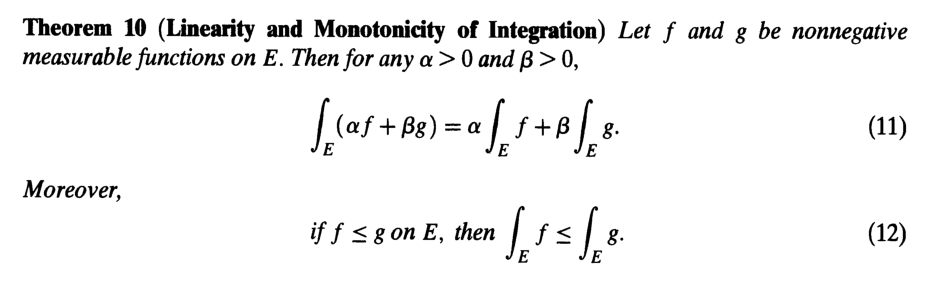
\includegraphics[width=\textwidth]{4-hw11-2025052023.png}
% \caption{}
\label{}
\end{figure}
\begin{figure}[H]
\centering
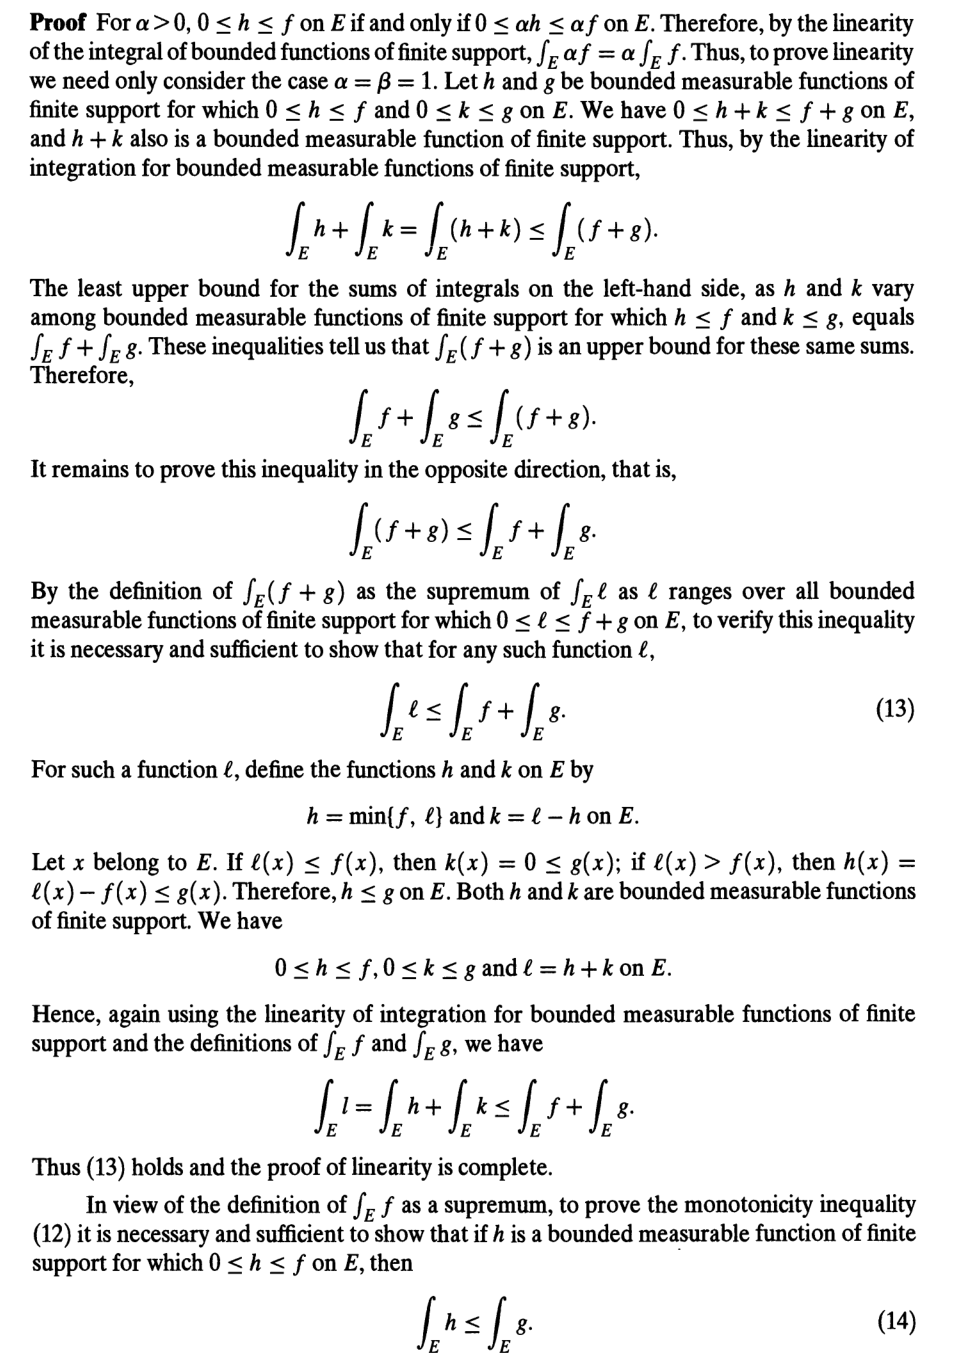
\includegraphics[width=\textwidth]{5-hw11-2025052023.png}
% \caption{}
\label{}
\end{figure}
\begin{figure}[H]
\centering
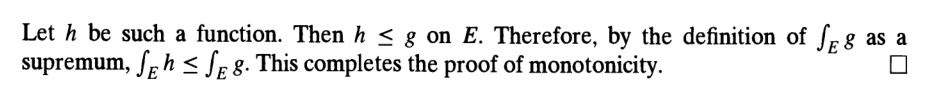
\includegraphics[width=\textwidth]{6-hw11-2025052023.png}
% \caption{}
\label{}
\end{figure}

\begin{figure}[H]
\centering
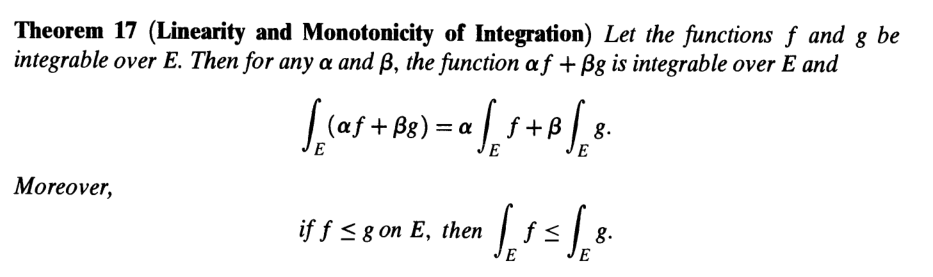
\includegraphics[width=\textwidth]{7-hw11-2025052023.png}
% \caption{}
\label{}
\end{figure}

\begin{figure}[H]
\centering
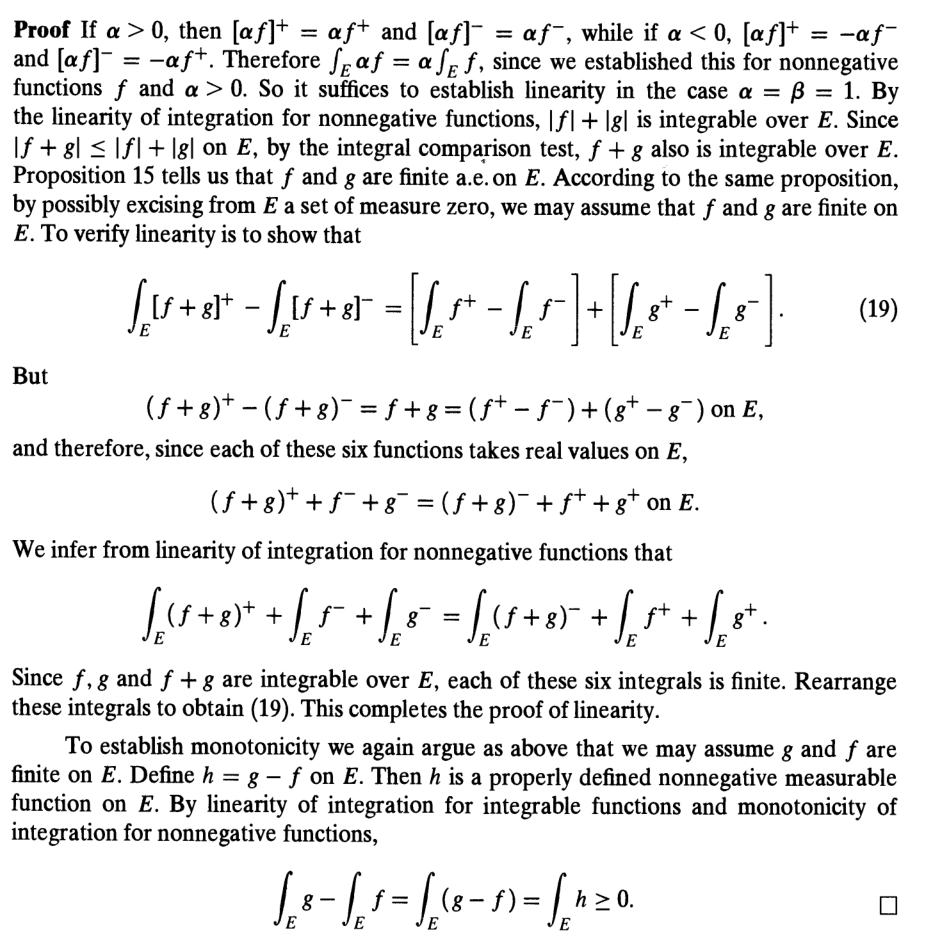
\includegraphics[width=\textwidth]{8-hw11-2025052023.png}
% \caption{}
\label{}
\end{figure}

\end{proof}
